\section[Prototipação]{Prototipação}

A prototipação não seria utilizada, até deparar-se com o problema de não saber como seria a imagem final das telas, então optou-se por utilizar a prototipagem de baixa fidelidade, onde o importante seria ter uma noção geral de como seriam as telas. Desenhou-se então no papel um exemplo de como imaginava-se que seria a tela final do jogo. O primeiro desenho foi o seguinte

\begin{figure}[H]
\centering
\caption{Prototipação das telas iniciais do jogo}
\label{prot0}
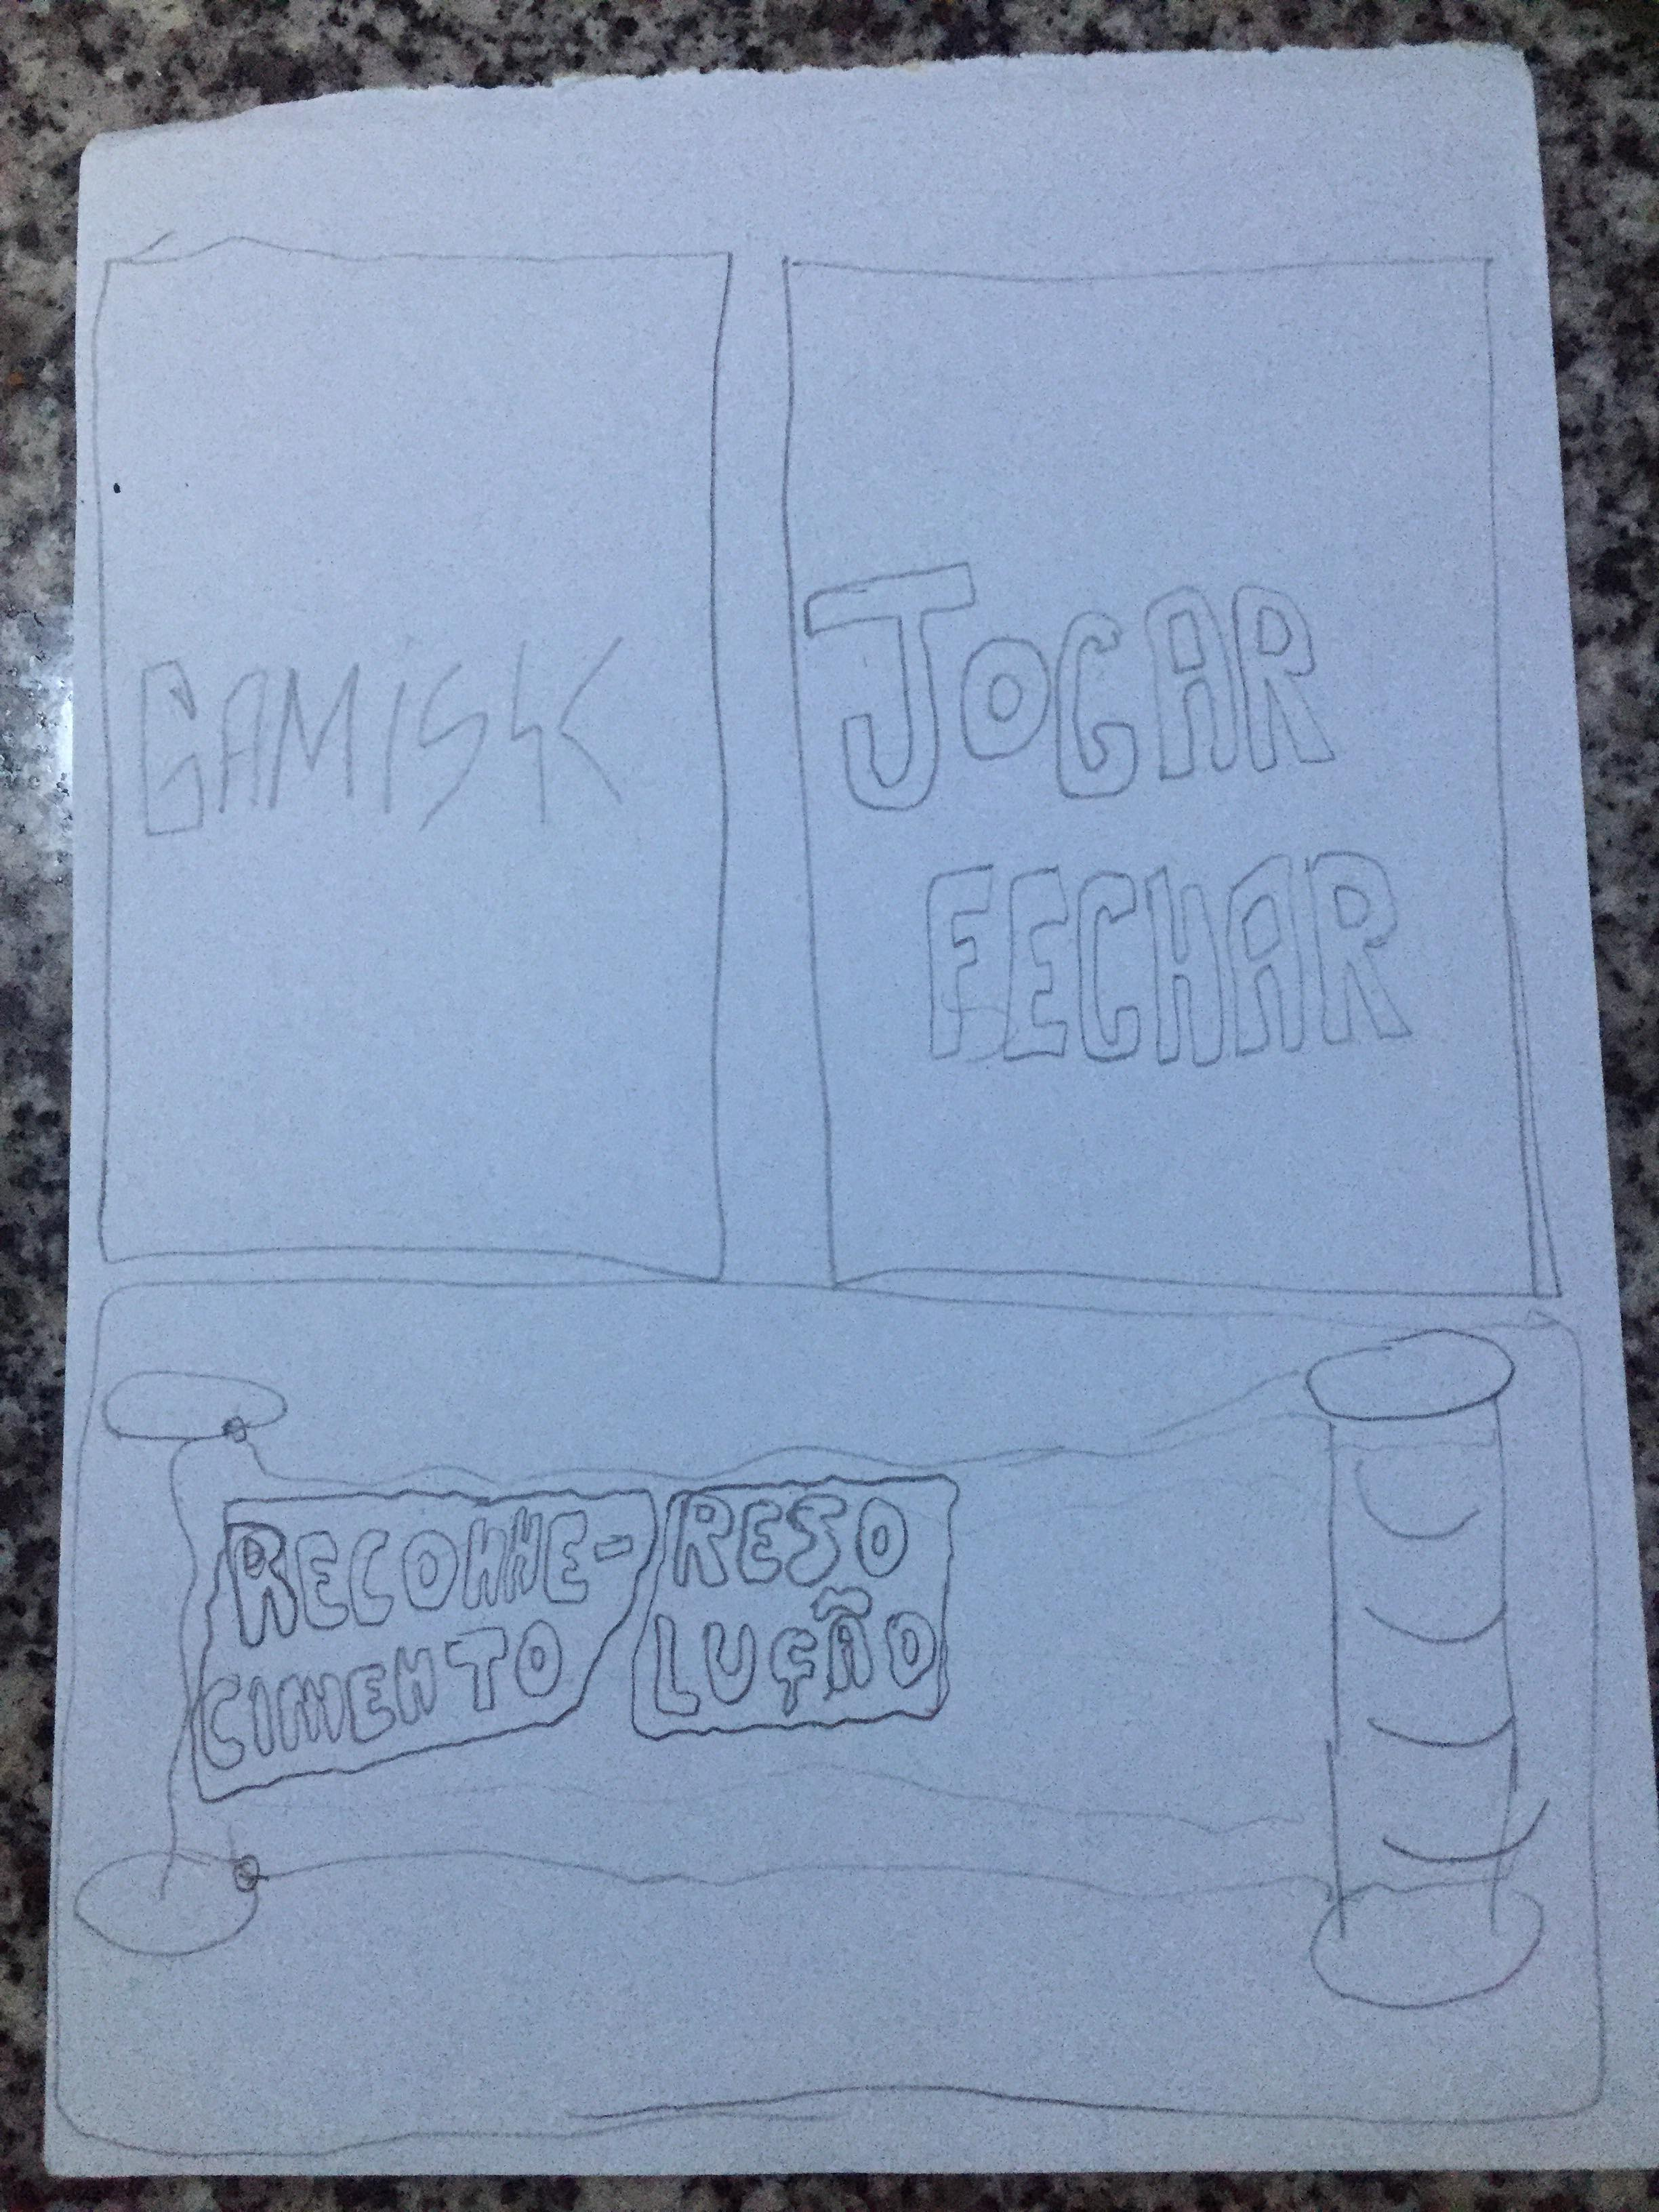
\includegraphics[scale=0.14]{figuras/prot0.jpg}
\\
\small{Fonte: do próprio autor}
\end{figure}

Na Figura \ref{prot0} no primeiro retângulo em cima e à esquerda é possível ver escrito "Gamisk", que seria o primeiro nome do jogo e a primeira tela a ser apresentada ao clicar no ícone do APP. Ao lado do retângulo Gamisk à direita é possível ver escrito "Jogar" e "Fechar" que seria a segunda tela do jogo. Porém percebeu-se que não haveria necessidade das duas telas e então decidiu-se pular direto para a que apresenta "RECONHECIMENTO" E "RESOLUÇÃO". A necessidade da tela gamisk seria em caso do jogo demorar para carregar recursos, o que não acontece. A necessidade da segunda tela era para ter o botão fechar, para o jogador poder sair do jogo, porém os celulares android apresentam o botão "Home" para sair da aplicação, então viu-se desnecessário criar a funcionalidade de sair do jogo. Então ao abrir o APP o usuário já será redirecionado para escolher o módulo de jogo que deseja jogar.


A Figura \ref{prot2} retrata como seria o jogo enquanto pensava-se que existiria os níveis de dificuldades fácil, médio e difícil. Depois houve o mapeamento dos níveis de dificuldade para o indicado na Figura \ref{prot1}. A mudança foi então que ao invés das fases terem nome 'fácil', 'médio' e 'difícil', elas passaram a ter o nome de 'ordem', 'homogeneidade', 'tipo' e 'linearidade' e foram ordenadas de acordo com o que acreditava-se ser mais fácil para classificar até o mais difícil.


\begin{figure}[H]
\centering
\caption{Prototipação das telas dos módulos}
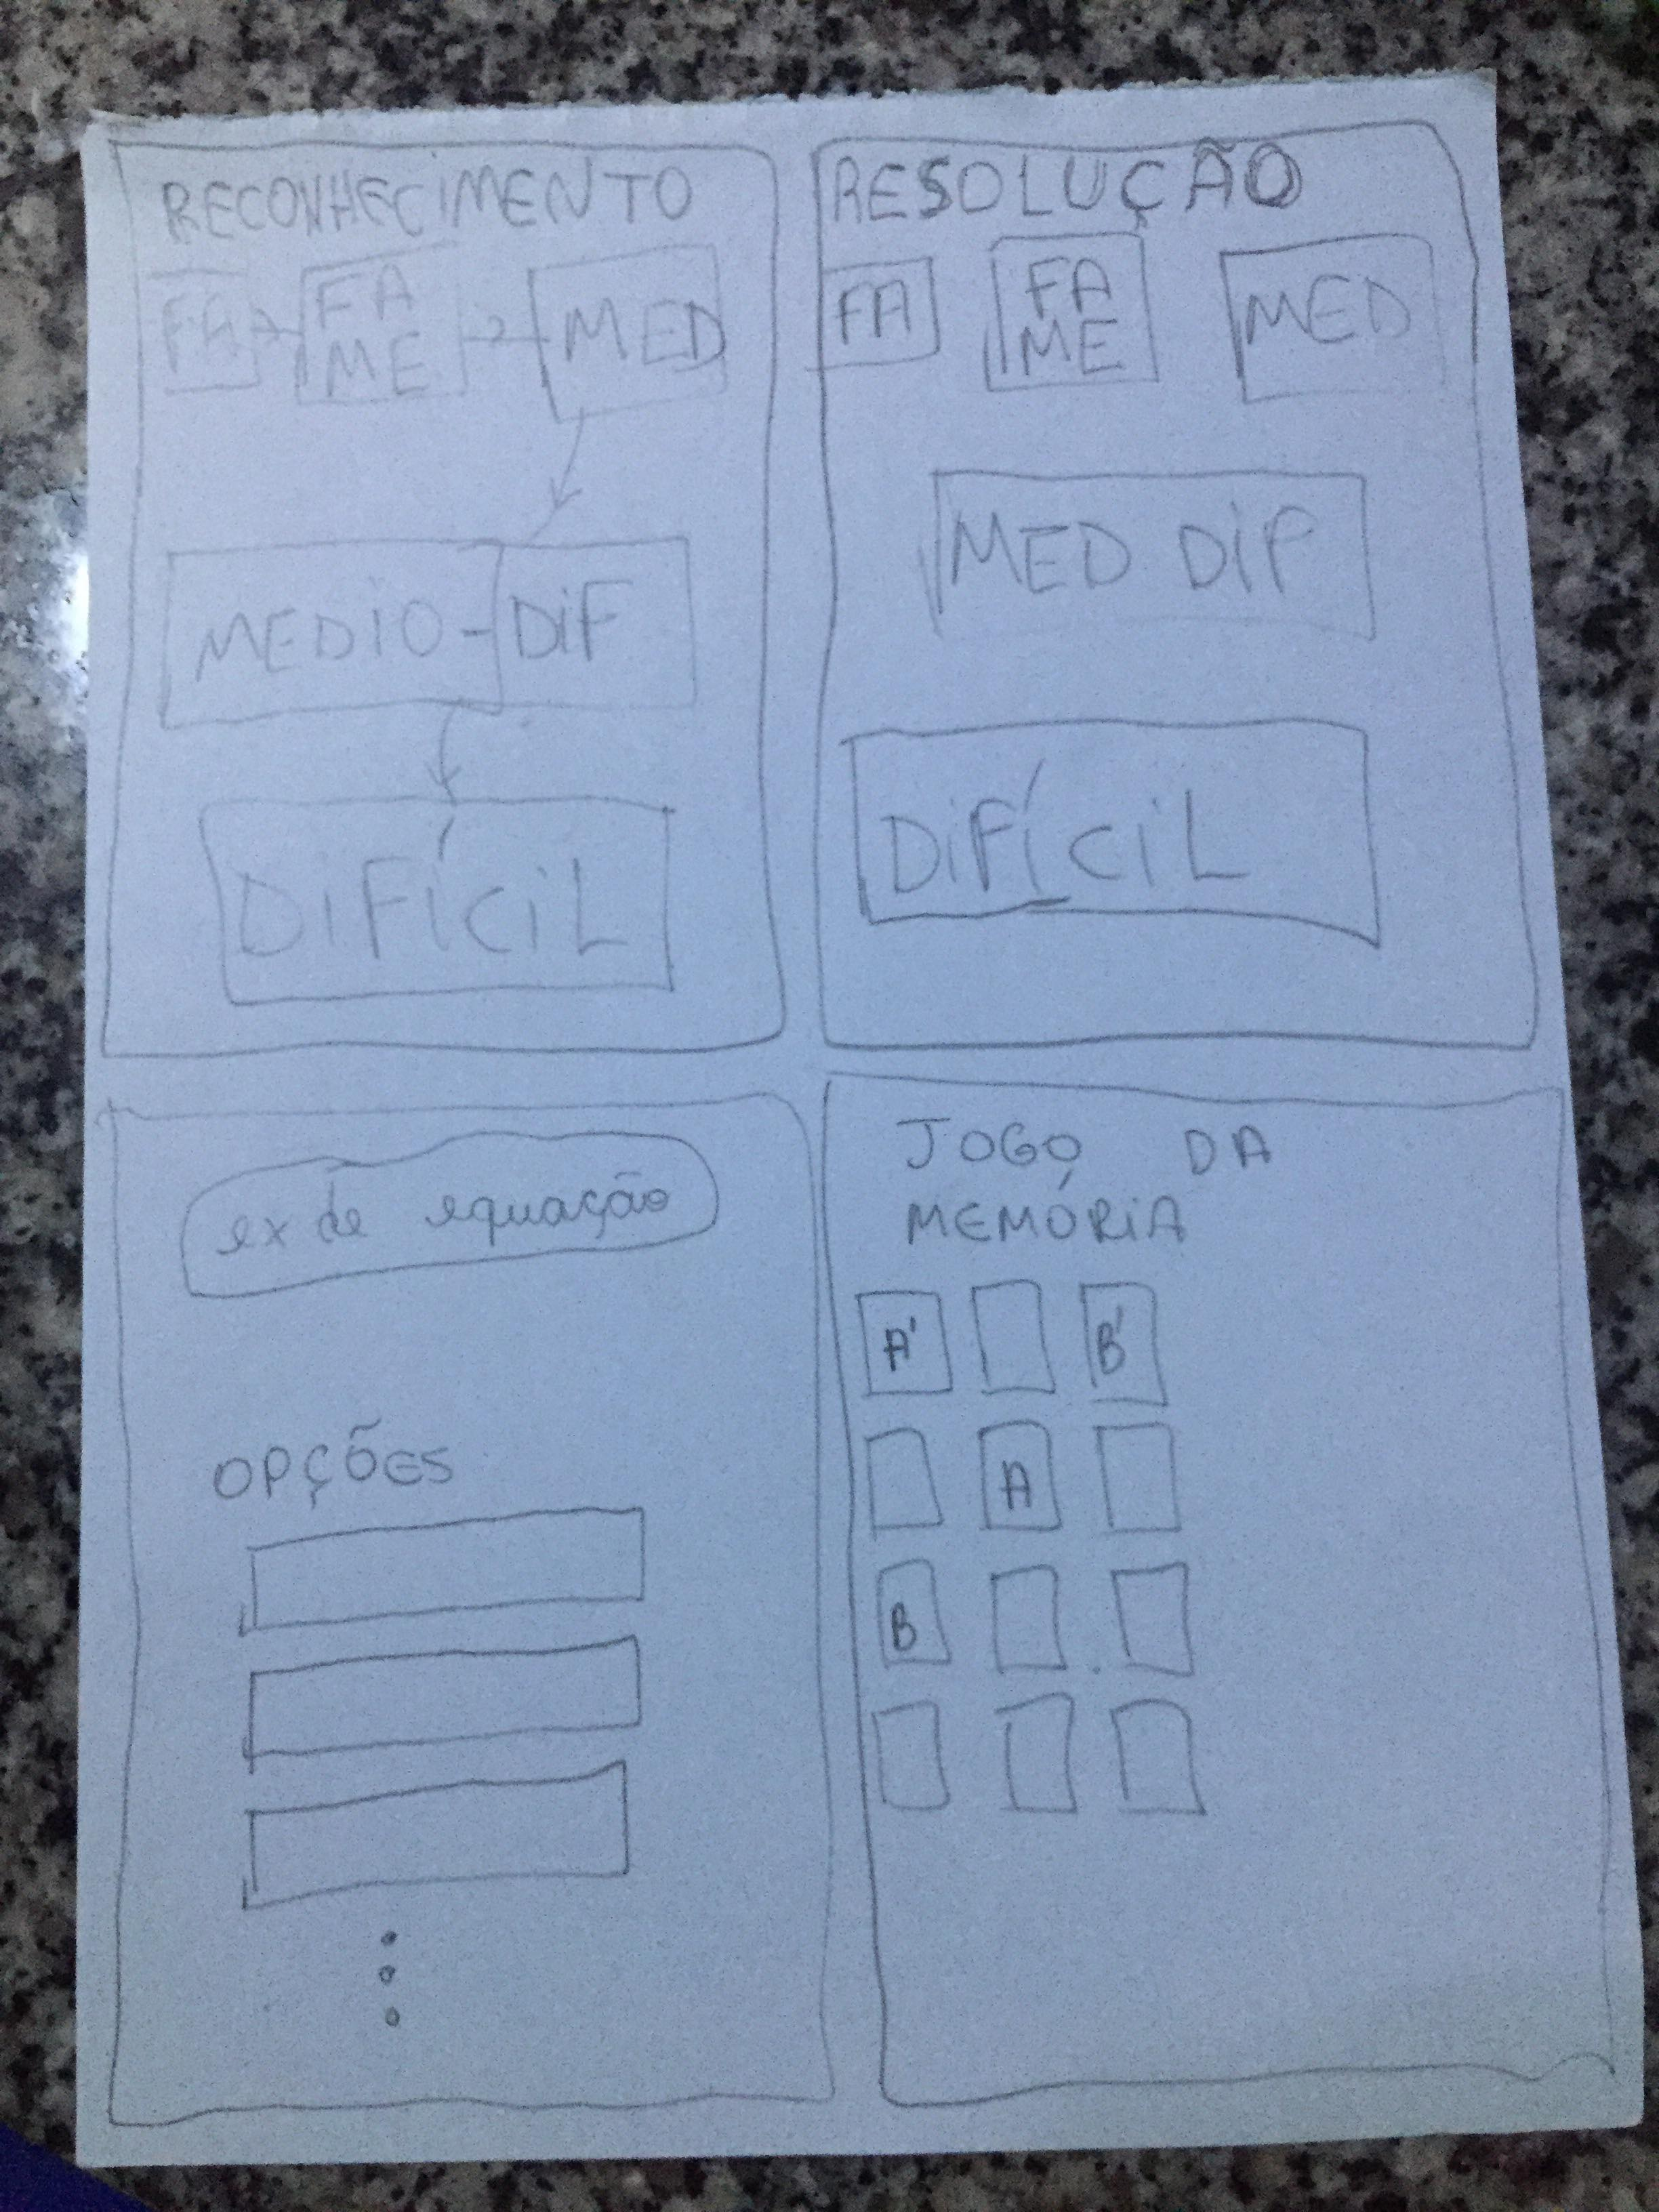
\includegraphics[scale=0.13]{figuras/prot2.jpg}
\label{prot2}
\\
\small{Fonte: do próprio autor}
\end{figure}

A imagem do jogo da memória acima onde tem o par \textit{A, A'} e \textit{B, B'} teve de ser redimensionada pelo tamanho das imagens não ficar legível apenas no desenho das cartas. Para isso a criação de duas telas para mostrar as duas equações \textit{clickadas} com maior clareza. É possível ver a nova tela na Figura \ref{prot3}

\begin{figure}[H]
\centering
\caption{Nova tela de resolução}
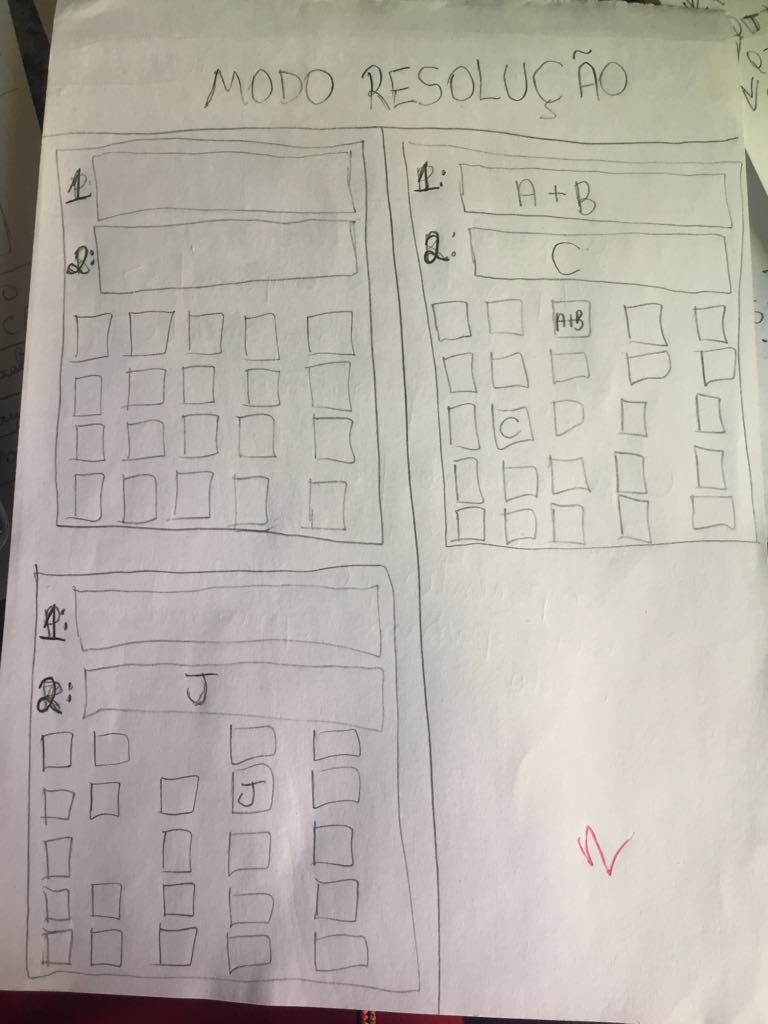
\includegraphics[scale=0.53]{figuras/prot3.jpg}
\label{prot3}
\\
\small{Fonte: do próprio autor}
\end{figure}


\begin{figure}[H]
\centering
\caption{Prototipação das telas dos módulos}
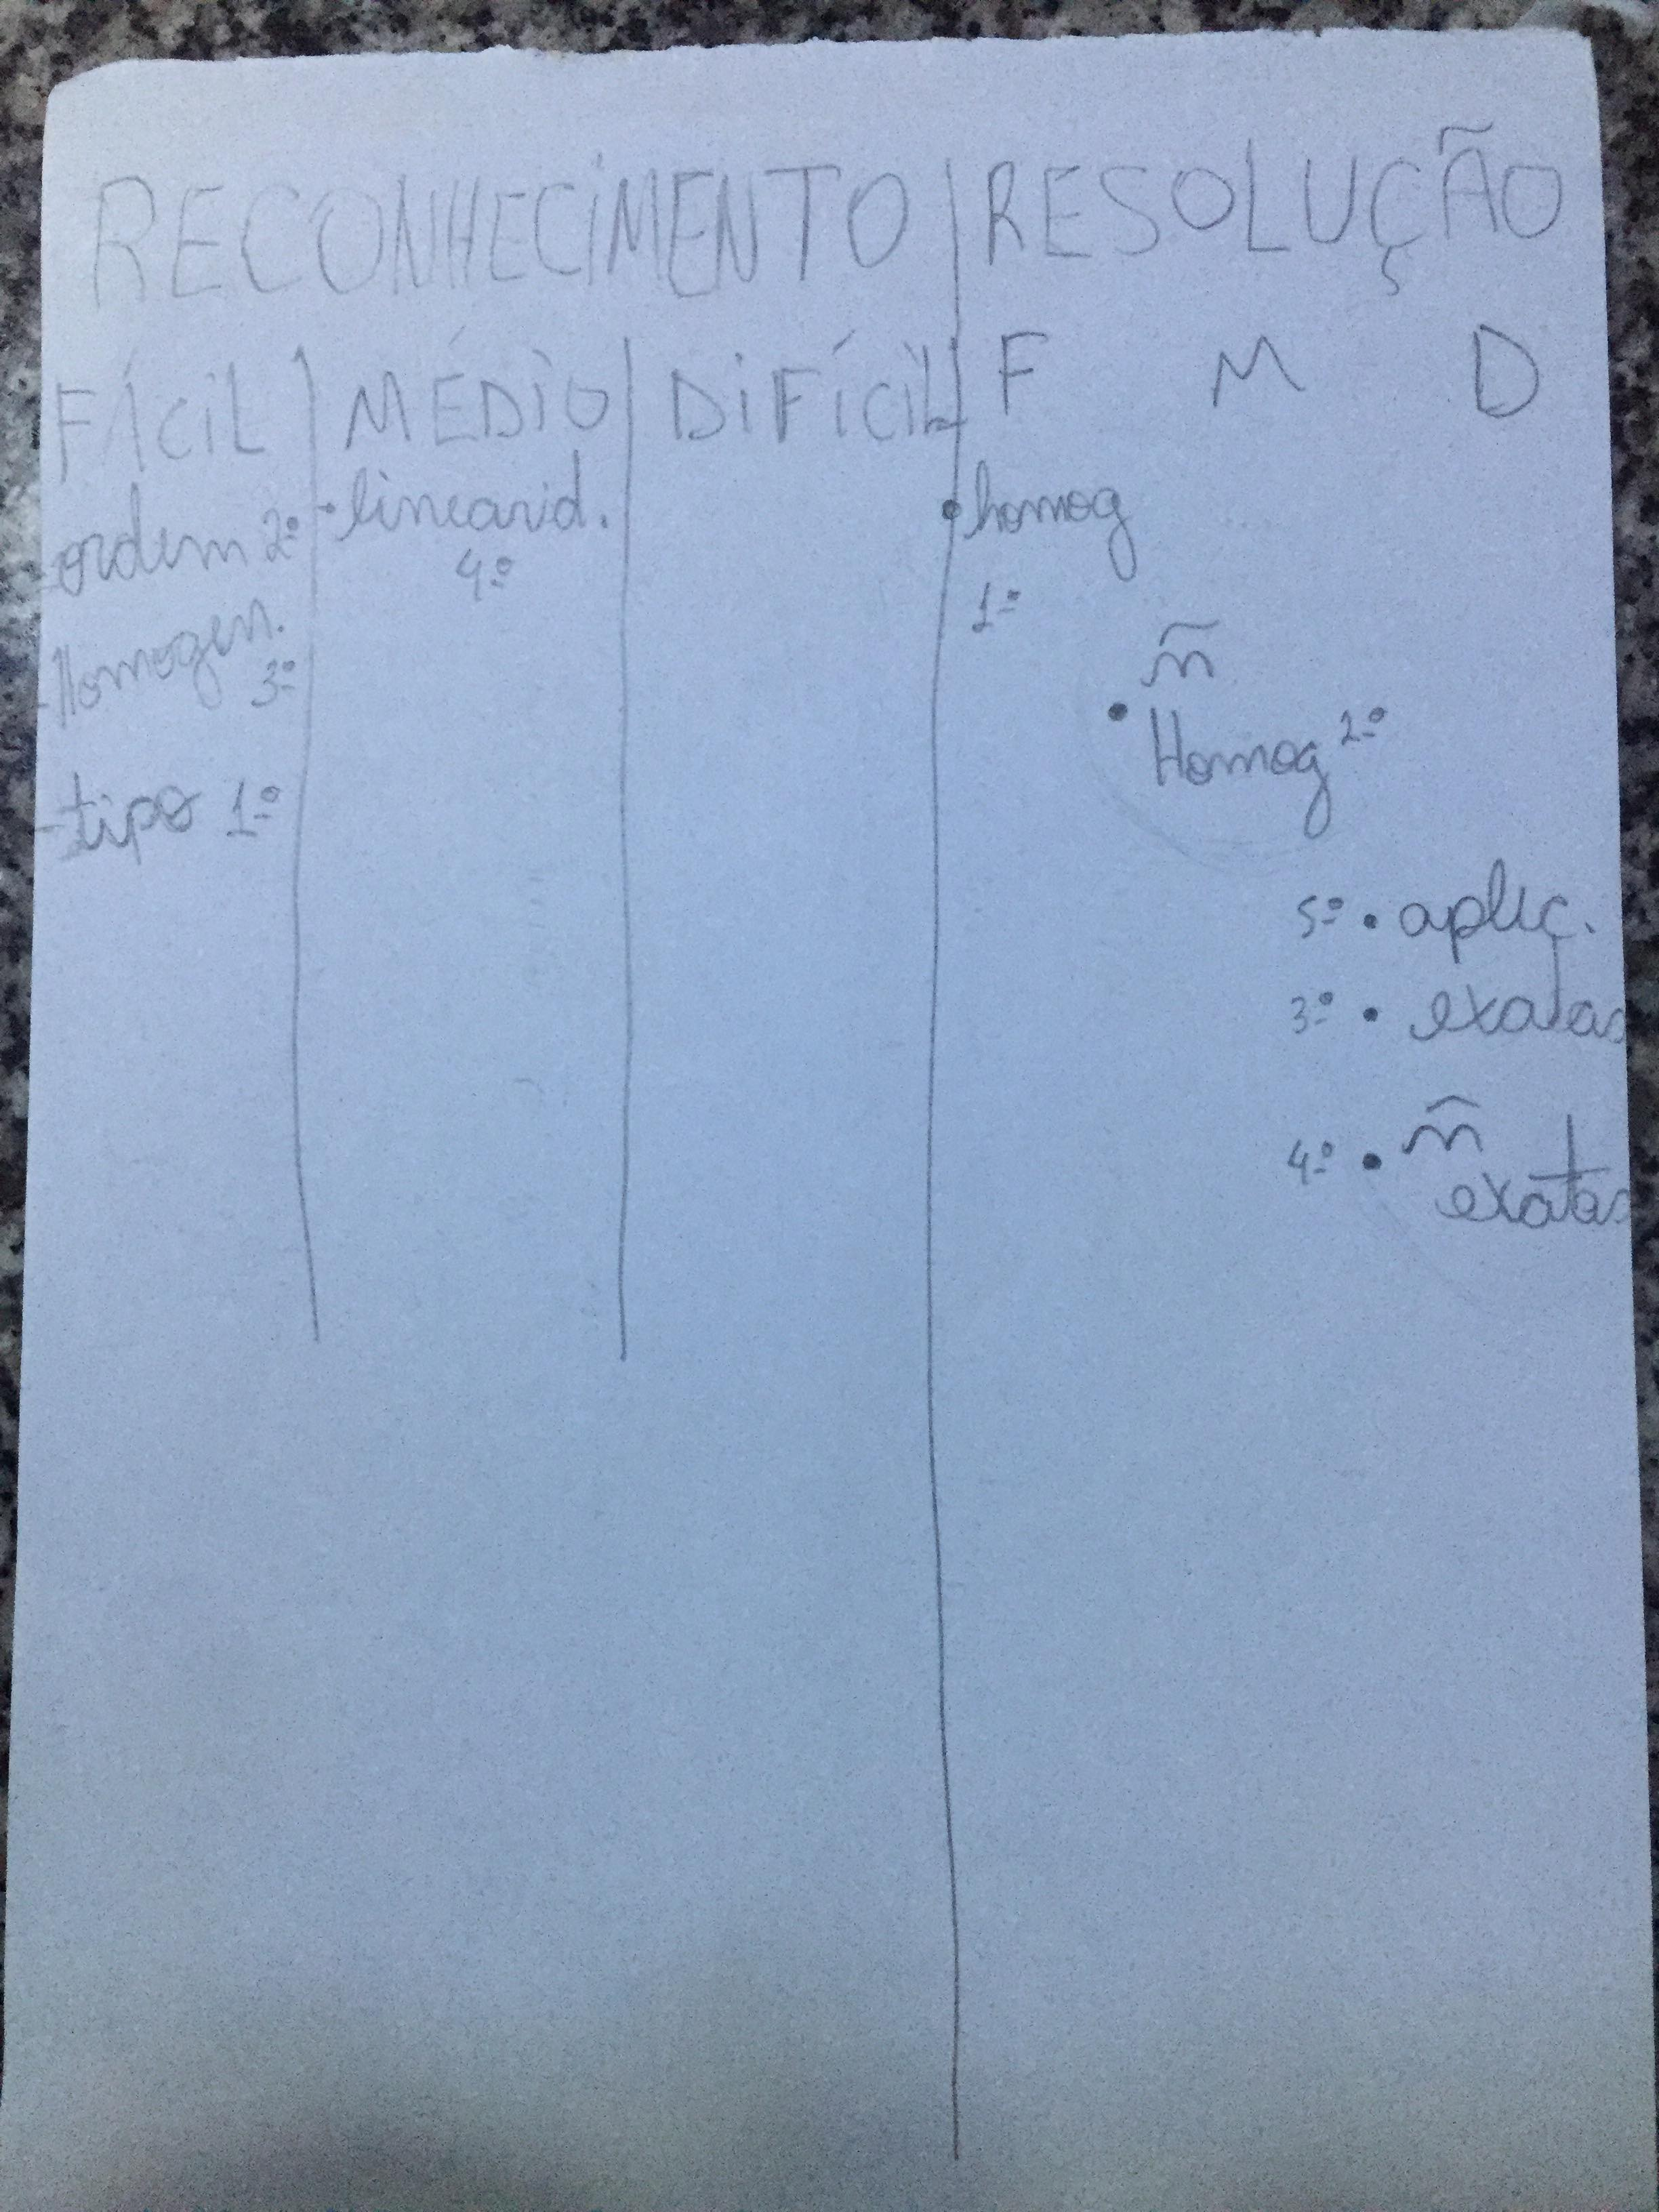
\includegraphics[scale=0.13]{figuras/prot1.jpg}
\label{prot1}
\\
\small{Fonte: do próprio autor}
\end{figure}
